\documentclass[11 pt,russian]{article}
\hoffset=-2cm \voffset=-2.5cm \textwidth=17cm \textheight=23cm

\usepackage[utf8]{inputenc}
\usepackage[russian]{babel}
\usepackage{amssymb, amsfonts, amsthm, amsmath}
\usepackage{graphicx}
\DeclareGraphicsRule{*}{mps}{*}{}

\newcounter{variant}
\newcounter{zadacha}[variant]

\newcommand{\z}{\par \addtocounter{zadacha}{1}\textbf{Вариант \Roman{variant} №\arabic{zadacha}.} }

\newcommand{\gr}{^\circ}

\newcommand{\Solution}{\ \\\noindent Решение.\\}
\newcommand{\Answer}[1]{Ответ: #1.\\}

\newcommand{\tasknumber}[2]{\ \\\noindent\textbf{#1 год. №#2.}}


\newcommand*{\hm}[1]{#1\nobreak\discretionary{}%
{\hbox{$\mathsurround=0pt #1$}}{}}
%для 10 задачи
\newcounter{num}

\newcommand{\n}{\par\addtocounter{num}{1}%
\textbf{\arabic{num}.}\ }

%\linespread{0.2}

%=============================================

\begin{document}

\tasknumber{2018}{1} Решить уравнение: $x^3-x^2+4x-4=0$.

\Solution Разложим левую часть уравнения на множители методом группировки.
\begin{center}
$x^3-x^2+4x-4=0 \Leftrightarrow x^2\cdot (x-1)+4\cdot (x-1)=0 \Leftrightarrow (x^2+4)\cdot (x-1)=0 \Leftrightarrow \left[
\begin{array}{l}
x^2+4=0,\\
x-1=0.
\end{array}
\right.\Leftrightarrow x-1=0 \Leftrightarrow x=1.$
\end{center}
\Answer{$\{1\}$}

\hrule
\tasknumber{2018}{2} Упростить: $\dfrac{a^2-1}{3a^2-4a+1}\cdot\dfrac{3a-1}{a}-\dfrac{1}{a}.$
\Solution Разложим на множители знаменатель первой дроби, после чего приведем дроби к общему знаменателю:
\begin{center}
$\dfrac{a^2-1}{3a^2-4a+1}\cdot\dfrac{3a-1}{a}-\dfrac{1}{a}\hm=\dfrac{(a+1)(a-1)(3a-1)}{3(a-1)\left(a-\frac{1}{3}\right)a}-\dfrac{1}{a}\hm=\dfrac{(a+1)(3a-1)}{(3a-1)a}-\dfrac{1}{a}\hm=\dfrac{a+1}{a}-\dfrac{1}{a}\hm=\dfrac{a+1-1}{a}\hm=\dfrac{a}{a}\hm=1.$
\end{center}
\Answer{$1$}
\hrule
\tasknumber{2018}{3} В шахматном турнире принимали участие 15 шахматистов, причем каждый из них сыграл только одну партию с каждым из остальных. Сколько всего партий было сыграно в этом турнире?

\Solution Рассмотрим первого шахматиста. По условию он сыграл одну партию с каждым из участников, тогда всего у него было 14 партий.\\
Рассмотрим второго шахматиста. Он также сыграл 14 партий, но партию с первым участником мы уже посчитали, тогда надо посчитать ещё 13 партий.\\
Рассуждая аналогично, понимаем что надо найти $S=\sum\limits_{n=1}^{14}n$ = 105.\\
\Answer{105 партий}
\hrule
\tasknumber{2018}{4} Решить уравнение: $(x^2-2x)^2-2x^2+4x=3$.

\Solution Выделим в левой части полный квадрат:
\begin{center}
$(x^2-2x)^2-2x^2+4x=3 \Leftrightarrow(x^2-2x)^2-2(x^2-2x)\hm=3 \Leftrightarrow (x^2-2x)^2-2(x^2-2x)+1\hm=4 \hm \Leftrightarrow (x^2-2x-1)^2\hm=4 \hm\Leftrightarrow \left[
\begin{array}{l}
x^2-2x-1=2,\\
x^2-2x-1=-2
\end{array} 
\right. \hm\Leftrightarrow \left[
\begin{array}{l}
x^2-2x-3=0,\\
x^2-2x+1=0
\end{array} 
\right.\hm \Leftrightarrow \left[
\begin{array}{l}
(x-3)(x+1)=0,\\
(x-1)^2=0
\end{array} 
\right.\hm \Leftrightarrow \left[
\begin{array}{l}
x=3,\\
x=-1,\\
x=1.
\end{array} 
\right. $ 
\end{center}

\Answer{$\{-1;1;3\}$}

\hrule
\tasknumber{2018}{5} Решить неравенство: $\dfrac{x^2-2x-8}{x-4}\leq7.$
\Solution Перенесем все влево и приведем к общему знаменателю:
\begin{center}
$\dfrac{x^2-2x-8}{x-4}\leq7 \Leftrightarrow \dfrac{x^2-2x-7x-8+28}{x-4}\leq0 \Leftrightarrow \dfrac{x^2-9x+20}{x-4}\leq0.$\\
\end{center}
По теореме Виета найдем корни числителя и разложим его по теореме Безу.
\begin{center}
$x^2-9x+20=0 \Leftrightarrow  \left[
\begin{array}{l}
    x=4,\\
    x=5.
  \end{array}
\right. \Leftrightarrow (x-4)(x-5)=0$
\end{center}
Вернёмся к неравенству:
\begin{center}
$\dfrac{(x-4)(x-5)}{x-4}\leq0 \Leftrightarrow \left\{
\begin{array}{l}
x-5\leq0,\\
x\neq4
\end{array} \right. \Leftrightarrow \left\{
\begin{array}{l}
x\leq5,\\
x\neq4.
\end{array} \right.$
\end{center}
\Answer{$(-\infty; 5]\setminus\{4\}$}

\hrule
\tasknumber{2018}{6} Решить систему: $
\left\{
\begin{array}{l}
0.4x+\dfrac{1}{3}y=1.8,\\
\dfrac{1}{5}x+0.27y=1.21.
\end{array}
\right.
$
\Solution
Выразим $x$ из второго уравнения и подставим в первое:
\begin{center}$
\left\{
\begin{array}{l}
0.4x+\dfrac{1}{3}y=1.8,\\
\dfrac{1}{5}x+0.27y=1.21
\end{array}
\right. \hm\Leftrightarrow
\left\{
\begin{array}{l}
0.4x+\dfrac{1}{3}y=1.8,\\
x=6.05-1.35y
\end{array}
\right. \hm\Leftrightarrow
\left\{
\begin{array}{l}
0.4\cdot (6.05-1.35y)+\dfrac{1}{3}y=1.8,\\
x=6.05-1.35y
\end{array}
\right. \hm\Leftrightarrow
\left\{
\begin{array}{l}
\dfrac{121}{50}-\dfrac{27}{50}y+\dfrac{1}{3}y=\dfrac{9}{5},\\
x=6.05-1.35y
\end{array}
\right. \hm\Leftrightarrow
\left\{
\begin{array}{l}
y=3,\\
x=6.05-1.35\cdot 3.
\end{array}
\right. \hm\Leftrightarrow
\left\{
\begin{array}{l}
y=3,\\
x=2.
\end{array}
\right.$
\end{center}
\Answer {$(x;y)\in\{(2;3)\}$}

\hrule
\tasknumber{2018}{7} Решить уравнение $|x-7|+|x-5|=x-4$\\
Построим на числовой оси знаки раскрытия модулей в зависимости от $x$\\
\begin{center}
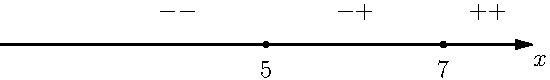
\includegraphics[scale =1]{7.pdf}\\
\end{center}
Разберем три случая.\\
\noindent
1) Пусть $x\leqslant5$. Тогда уравнение принимает вид:
\begin{center}
$-x+7-x+5=x-4 \Leftrightarrow -3x=-16\Leftrightarrow x=\dfrac{16}3.$\\
\end{center}
Так как $\frac{16}3>5$, то найденный корень $x=\frac{16}3$ -- не подходит под условие случая.\\[0.3cm]
\noindent
2) $5<x<7$\\
$-x+7+x-5=x-4 \Leftrightarrow x=6$\\
$5<6<7 \Rightarrow x=6 - \text{подходит.}$\\[0.3cm]
\noindent
3) $x\geqslant 7$\\
$x-7+x-5=x-4 \Leftrightarrow x=8$\\
$8\geqslant7 \Rightarrow x=8 - \text{подходит.}$\\

\Answer{\{6;8\}}

\hrule
\tasknumber{2018}{8} Вычислить: $(2-\sqrt{5})(\sqrt{9+4\sqrt{5}})$
\Solution
Выделим в подкоренном выражении второго корня полный квадрат:
\begin{center}
$(2-\sqrt{5})(\sqrt{9+4\sqrt{5}})=(2-\sqrt{5})(\sqrt{5+4\sqrt{5}+4})=(2-\sqrt{5})\left(\sqrt{(2+\sqrt{5})^2}\right)\hm=(2-\sqrt{5})(2+\sqrt{5})\hm=4-5\hm=-1$
\end{center}
\Answer{$-1$}
\hrule
\tasknumber{2018}{9} Построить график: $y=\dfrac{|x^2-5x+6|}{x-2}$\\
\begin{center}
Разложим числитель на множители по теореме Безу:
$x^2-5x+6=(x-2)(x-3) \hm\Rightarrow$\\
При $ x \in (-\infty; 2)\cup (3; +\infty): (x-2)(x-3)\geqslant 0,$ при $ x \in (2;3]: (x-2)(x-3)<0 $\\
1)При $x \in (-\infty; 2)\cup (3; +\infty): y=\dfrac{(x-2)(x-3)}{x-2} \Leftrightarrow \left\{
\begin{array}{l}
y=x-3,\\
x\neq2.
\end{array} 
\right. $\\
2)При $x \in (2;3], y=-\dfrac{(x-2)(x-3)}{x-2}\Leftrightarrow \left\{
\begin{array}{l}
y=3-x,\\
x\neq2.
\end{array} \right.$\\
 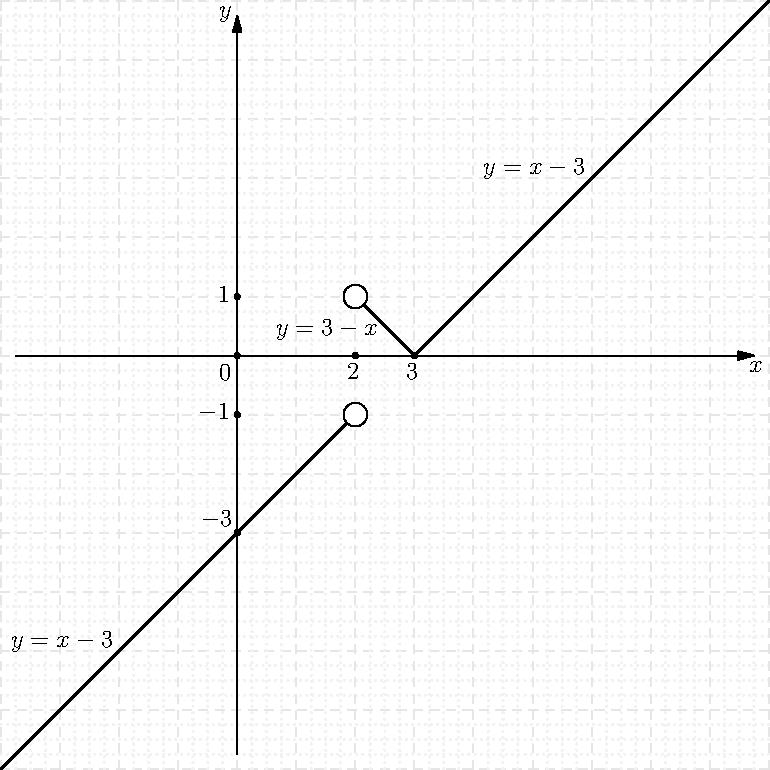
\includegraphics[scale =1]{graphic.pdf}
\end{center}
\hrule
\tasknumber{2018}{10} Найдите все значения параметра $a$, при которых сумма корней уравнения\\ $x^2-\left(a^2-5a\right)x+4a^2=0$  будет отрицательной.\\
\Solution
\n Чтобы уравнение $x^2-\left(a^2-5a\right)x+4a^2=0$ имело корни, сумма которых была бы меньше $0$, необходимо и достаточно, чтобы\\
1) Уравнение имело один корень, который был бы меньше $0$.\\
ИЛИ\\
2) Имело 2 корня, сумма которых была бы меньше $0$.
\\
\\\n Рассмотрим первый случай. Т.к. уравнение всегда квадратное (старший коэффициент не равен нулю), то надо рассмотреть случай, когда дискриминант равен нулю:
\begin{center}
$(a^2-5a)^2-4\cdot4a^2=0\Leftrightarrow a^4-10a^3+25a^2-16a^2=0 \Leftrightarrow a^4-10a^3+9a^2=0 \Leftrightarrow a^2-10a+9 = 0 \hm\Leftrightarrow a=5\pm\sqrt{25-9} \hm\Leftrightarrow a=5\pm\sqrt{16} \hm\Leftrightarrow a=5\pm4\Leftrightarrow \left[ 
\begin{array}{l}
a=1,\\
a=9. 
\end{array} \right.$
\end{center}
Подставим $a=1$ в изначальное уравнение:\\
\begin{center}
$x^2-(1^2-5\cdot1)x+4\cdot1^2=0\Leftrightarrow x^2+4x+4 = 0\Leftrightarrow (x+2)^2 = 0\Leftrightarrow x=-2.$\\
$-2<0 \Rightarrow a=1 - \text{подходит}.$\\\end{center}
Подставим $a=9$ в изначальное уравнение:\\
\begin{center}
$x^2-(9^2-5\cdot9)x+4\cdot9^2=0\Leftrightarrow x^2-36x+324 = 0\Leftrightarrow (x-18)^2=0\Leftrightarrow x=18.$\\
$18>0\Rightarrow a=9 - \text{не подходит}.$\\\end{center}
\n Рассмотрим второй случай.\\
Чтобы было два корня, необходимо, чтобы дискриминант был больше нуля:
\begin{center}
$(a^2-5a)^2-4\cdot4a^2 > 0\Leftrightarrow a^4-10a^3+25a^2-16a^2 > 0\Leftrightarrow a^4-10a^3+9a^2 > 0\Leftrightarrow a^2-10a+9 > 0\hm\Leftrightarrow (a-1)(a-9)>0.$
	\end{center}
По теореме Виета: $x_1+x_2=\dfrac{a^2-5a}{1}$, где $x_1$ и  $x_2$ -- корни изначального уравнения.\\
Тогда, необходимо и достаточно, чтобы выполнялась система: $\left\{
\begin{array}{l}
a^2-5a<0,\\
(a-1)(a-9)>0.
\end{array} \right.$\\
Решим её методом интервалов:\\
\begin{center}$
\left\{ \begin{array}{l}
a^2-5a<0,\\
(a-1)(a-9)>0
\end{array} \right. \Leftrightarrow
\left\{ \begin{array}{l}
a(a-5)<0,\\
(a-1)(a-9)>0
\end{array} \right. \Leftrightarrow
\left\{ \begin{array}{l}
a\in(0;5),\\
a\in(-\infty;1)\cup(9;+\infty)
\end{array} \right. \Leftrightarrow a\in\left(0;1\right).
$\end{center}
Объединим оба случая и получим $a\in\left(0;1 \right]$.\\
\Answer{$a\in\left(0;1 \right]$}

\hrule
\tasknumber{2018}{12} Остаток от деления числа $a$ на $3$ равен $1$. Найдите отстаток от деления числа $a^2$ на $3$.
\Solution Если остаток от деления числа  $a$ на $3$ равен $1$, то число $a$ можно записать в виде $a=3k+1,$ где $k$ -- это какое-то целое число.\\
Тогда $a^2 = (3k+1)^2 = 9k^2+6k+1 = 3(3k^2+2k)+1.$ Поскольку первое слагаемое делится на $3$, то остаток от деления $a^2$ на $3$ будет равен $1$.\\
\Answer{$1$}


\hrule
\tasknumber{2018}{14} При каких $a$ уравнение $(x-3)(2x-a)=x-3$ имеет ровно один корень?
\Solution Раскроем скобки и перенесем всё в левую часть: \begin{center}
$2x^2-ax-6x+3a=x-3.
2x^2-x(7+a)+3a+3=0.$\end{center}
Т.к уравнение всегда квадратное (старший коэффициент не равен нулю) то, чтобы уравнение имело ровно один корень, необходимо и достаточно, чтобы дискриминант был равен $0$, то есть:
\begin{center}
$(7+a)^2-8(3a+3)=0. \Leftrightarrow 49+14a+a^2-24a-24=0.\Leftrightarrow a^2-10a+25=0 \Leftrightarrow (a-5)^2=0 \Leftrightarrow a=5.$\\
\end{center}
\Answer{$a=5$}


\end{document}